\documentclass[]{article}

\usepackage{tikz}
\usepackage{amsmath}
\usepackage{amsfonts}
\usepackage{amssymb}
\usepackage{relsize}
\usepackage{tkz-base}
\usepackage{tkz-euclide}

\usetikzlibrary{svg.path}
\usetikzlibrary{arrows}
\usetikzlibrary{shapes.geometric,calc}

\tikzset{
      ncbar/.style={
        to path=%
        ($(\tikztostart)!#1!90:(\tikztotarget)$)
        -- ($(\tikztotarget)!($(\tikztostart)!#1!90:(\tikztotarget)$)!90:(\tikztostart)$)
      },
      ncbar/.default=0.5cm,
    }
    
\newcommand{\crossout}[1]{\mathbin{\ooalign{${#1}$\cr\larger[1]{$\nearrow$}\cr}}}

%opening
\title{Kinematic Redundancy}
\author{Glen Henshaw\\Craig Carignan}



\begin{document}

\maketitle


\section{Formal Derivation of the Moore--Penrose Pseudo--Inverse }

Last time we discussed how using the Moore-Penrose pseudo--inverse was a way to bypass the difficulty with non--square Jacobians, and that it had some nice properties that made it particularly suitable as the basis for an inverse kinematics scheme. But we threw it up on the board as a magic formula. Now we're going to derive it, because understanding how to derive it will let you derive your own customized inverse kinematics schemes.

The fundamental approach is to treat the velocity--space kinematics problem as an optimization problem (sound familiar?):
\begin{displaymath}
\min \|\Delta \underline{q}\|_{2}^{2} \ \ \text{given}\ \ 	\Delta \underline{x} = J(\underline{q})\Delta\underline{q}
\end{displaymath}
We'll use Lagrangian multipliers, so we'll formulate the problem as follows:
\begin{displaymath}
C = \frac{1}{2} \Delta \underline{q}^{T}\Delta\underline{q} + \underline{\lambda}^{T}(\Delta\underline{x} - J\Delta\underline{q})
\end{displaymath}
to minimize this we must take the partial with respect to both $\Delta\underline{q}$ and $\Delta\underline{\lambda}$, set both equations to zero, and solve:
\begin{equation}
\frac{\partial C}{\partial \Delta\underline{q}} = \underline{0}^{T}= \Delta\underline{q}^{T} - \underline{\lambda}^{T}J \Rightarrow \Delta \underline{q} = J^{T}\underline{\lambda} \label{first}
\end{equation}
and
\begin{equation}
	\frac{\partial C}{\partial \Delta\underline{\lambda}} = \underline{0}^{T} = \Delta\underline{x}^{T} - \Delta\underline{q}^{T}J^{T} \Rightarrow \Delta \underline{x} = J \Delta\underline{q} \label{second}
\end{equation}
Substituting \ref{first} into \ref{second} gives
\begin{displaymath}
\Delta\underline{x}	= JJ^{T}\underline{\lambda} \Rightarrow \underline{\lambda}=(JJ^{T})^{-1}\Delta\underline{x}
\end{displaymath}
and substituting this into \ref{first} gives
\begin{equation}
\Delta\underline{q} = J^{T}(JJ^{T})^{-1}\Delta\underline{x} \triangleq J^{\dag} \Delta\underline{x}
\end{equation}
which gives us the result we want.

Note that you can change the initial optimization problem and derive different pseudo--inverses. For instance, you can add a term that penalizes distance from the arm to an object in the environment. Assume that $D(\underline{q} + \Delta\underline{q}\Delta t)$ is a positive, scalar function that has a ``hat'' shape with its maximum at a distance of zero and asymptotically approaches (or actually reaches) zero as the distance from the object increases. We can them write the following minimization problem:
\begin{displaymath}
\min \|\Delta \underline{q}\|_{2}^{2} + \gamma D(\underline{q} + \Delta\underline{q}\Delta t)\ \ \text{given}\ \ 	\Delta \underline{x} = J(\underline{q})\Delta\underline{q}
\end{displaymath}
We proceed as above:
\begin{displaymath}
C = \frac{1}{2} \Delta \underline{q}^{T}\Delta\underline{q} + \gamma D(\underline{q} + \Delta\underline{q}\Delta t)+ \underline{\lambda}^{T}(\Delta\underline{x} - J\Delta\underline{q})
\end{displaymath}
Take the partial with respect to both $\Delta\underline{q}$ and $\Delta\underline{\lambda}$, set both equations to zero, and solve:
\begin{equation}
\frac{\partial C}{\partial \Delta\underline{q}} = \underline{0}^{T} = \Delta\underline{q}^{T} + \gamma \frac{\partial D}{\partial \Delta\underline{q}}^{T}\Delta t - \underline{\lambda}^{T}J \Rightarrow \Delta \underline{q}  = J^{T}\underline{\lambda} - \gamma \frac{\partial D}{\partial \Delta\underline{q}}^{T}\Delta t \label{fourth}
\end{equation}
and
\begin{equation}
	\frac{\partial C}{\partial \Delta\underline{\lambda}} = \underline{0}^{T} = \Delta\underline{x}^{T} - \Delta\underline{q}^{T}J^{T} \Rightarrow \Delta \underline{x} = J \Delta\underline{q} \label{fifth}
\end{equation}

Substituting \ref{fourth} into \ref{fifth} gives
\begin{eqnarray}
    \Delta\underline{x}	& = & J\left[J^{T}\underline{\lambda} - \gamma \frac{\partial D}{\partial \Delta\underline{q}}^{T}\Delta t \right] \nonumber \\
    \Rightarrow JJ^{T}\underline{\lambda} & = & \Delta\underline{x} + \gamma J \frac{\partial D}{\partial \Delta\underline{q}}^{T}\Delta t \nonumber \\
    \Rightarrow \underline{\lambda} & = & (JJ^{T})^{-1}\left[\Delta\underline{x} + \gamma J \frac{\partial D}{\partial \Delta\underline{q}}^{T}\Delta t\right] \nonumber
\end{eqnarray}
and substituting this into \ref{fourth} gives
\begin{eqnarray}
    \Delta\underline{q} & = & J^{T}(JJ^{T})^{-1}\left[\Delta\underline{x} + \gamma J \frac{\partial D}{\partial \Delta\underline{q}}^{T}\Delta t\right] - \gamma \frac{\partial D}{\partial \Delta\underline{q}}^{T}\Delta t \nonumber \\
    & = & J^{\dag} \Delta\underline{x} + \gamma J^{\dag} J \frac{\partial D}{\partial \Delta\underline{q}}^{T}\Delta t  -\gamma \frac{\partial D}{\partial \Delta\underline{q}}^{T}\Delta t \nonumber \\
    & = & J^{\dag} \Delta\underline{x} + \left[J^{\dag}J - I\right] \frac{\partial D}{\partial \Delta\underline{q}}^{T}\Delta t 
\end{eqnarray}
Notice that this result is identical to the one above except for the addition of the strange partial derivative of the distance function. It turns out that $\left[J^{\dag}J - I\right]$ is a projection into the nullspace of $J$, i.e. we can choose any vector $\underline{r}$ and multiply it by the projection and it will not change the result:
\begin{displaymath}
   \Delta{x} = J(\underline{q})\Delta\underline{q} = J\left(\Delta\underline{q} + \left[J^{\dag}J - I\right] r\right)
\end{displaymath}
In practical terms, what we end up doing here is simultaneously fulfilling the tracking constraint $\Delta\underline{x} = J(\underline{q})\Delta\underline{q}$ and using whatever redundant degrees of freedom our arm has to move along the gradient away from the obstacle \textit{at the same time}. Recall our discussion last time about \textbf{self motion}: this technique uses the self motion of the robot arm to move away from a potential collision while maintaining end effector tracking. This may be an advantage or a disadvantage: the advantage is that you can guarantee that the end effector is exactly where you want it. The disadvantage is that if you command the end effector itself to collide with the environment, no amount of self motion can prevent a collision.

\section{Augmented Jacobian Approach}
Sometimes, we don't want our inverse kinematics routine to implicitly control the self motion of the arm; instead, we may want to control it directly. We can do this through augmenting the Jacobian. It can be augmented until it contains $\mathbb{N}-\mathbb{M}$ extra rows, making it square.

\begin{figure}[h!]
	\centering
	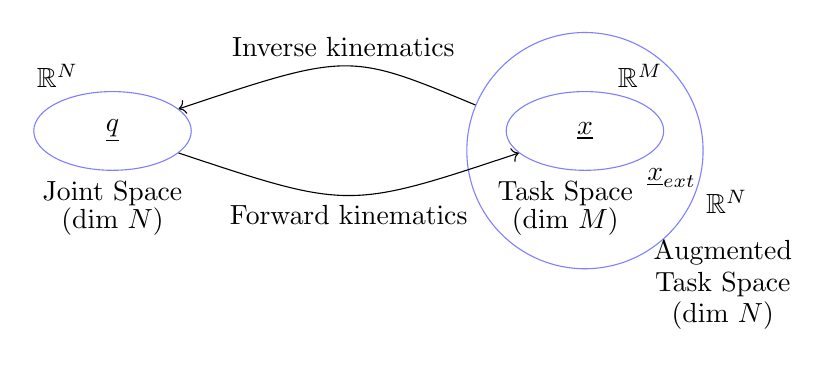
\begin{tikzpicture}
		\draw (0,0) node[shape=ellipse, draw=blue!50, minimum height=1cm, minimum width=2cm](angles){$\underline{q}$};
		\draw (-0.7,0.7) node{$\mathbb{R}^{N}$};
		\draw (0, -0.8) node{Joint Space};
		\draw (0, -1.15) node{(dim $N$)};
		\draw (6,-0.25) node[shape=ellipse, draw=blue!50, minimum height=3cm, minimum width=3cm](cart){};
		\draw (7.8,-0.9) node{$\mathbb{R}^{N}$};
        \draw (7.1,-0.6) node{$\underline{x}_{ext}$};
		\draw (7.75, -1.55) node{Augmented};
		\draw (7.75, -1.95) node{Task Space};
		\draw (7.75, -2.35) node{(dim $N$)};
		
		\draw (6,0) node[shape=ellipse, draw=blue!50, minimum height=1cm, minimum width=2cm](cart2){$\underline{x}$};
		\draw (6.7,0.7) node{$\mathbb{R}^{M}$};
		\draw (5.75, -0.8) node{Task Space};
		\draw (5.75, -1.15) node{(dim $M$)};
		
        \draw[->] (angles) .. controls (3, -1) .. (cart2) node[pos=0.5][below] {Forward kinematics};
		\draw[->] (cart) .. controls (3, 1) .. (angles) node[pos=0.5][above] {Inverse kinematics};

	\end{tikzpicture}
\end{figure}
The basic idea is that we are going to increase the dimensionality of ``task space'' to include not only end effector trajectories but trajectories in terms of other parts of our arm. If our original Jacobian relationship is
\begin{displaymath}
 \Delta\underline{x} = J_{\mathbb{M}\times\mathbb{N}}(\underline{q})\Delta\underline{q}
\end{displaymath}
where $\text{dim}(\underline{x}) = \mathbb{M}$ and $\text{dim}(\underline{q}) = \mathbb{N}$
then we're going to ``extend'' the Jacobian as follows:
\begin{displaymath}
 \underbrace{\left[ \begin{array}{c}\Delta\underline{x} \\ \Delta\underline{x}_{A}\end{array}\right]}_{\Delta\underline{x}_{ext}} = \underbrace{\left[ \begin{array}{c} J \\ J_{A} \end{array} \right]}_{J_{ext}} \Delta\underline{q}
\end{displaymath}
and our new Jacobian equation will be written as
\begin{eqnarray}
 \Delta\underline{x}_{ext} & = & J_{ext}\Delta\underline{q} \nonumber \\
 \Delta\underline{q} & = & J_{ext}^{-1}\Delta\underline{x}_{ext} \nonumber
\end{eqnarray}
\textbf{Note that we no longer need a pseudo--inverse} because our extended Jacobian is square. 

\subsection{7 DOF Anthropomorphic Arm}
Here's an example of how this works. This is a 7 DOF ``anthropomorphic'' arm, which means it has a three--axis shoulder, a pitch elbow, and a three--axis wrist. We want to control the motion of the end effector independently of the motion of the elbow's plane.

Here's a diagram:
\vspace{0.25in}
\begin{figure}[h!]
	\centering
	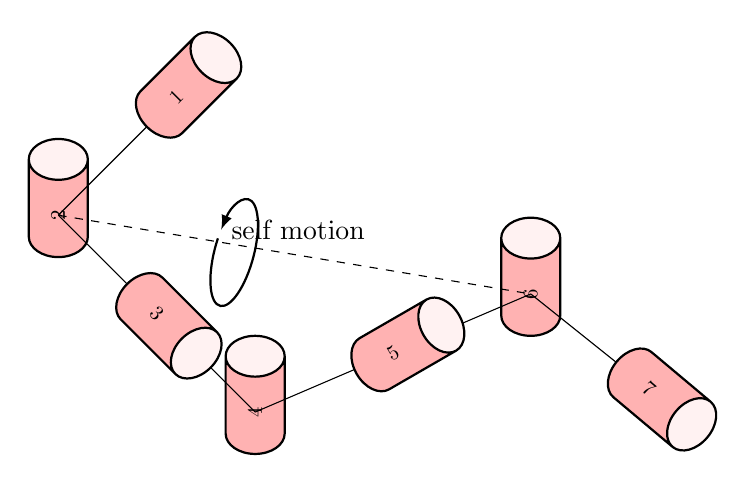
\begin{tikzpicture}
		
		\coordinate(A) at (2.5, 1.5);
		\coordinate(B) at (1,0);
		\coordinate(C) at (3.5, -2.5);
		\coordinate(D) at (7, -1);
		\coordinate(E) at (8.5, -2.2);
 
        \draw (B) node[cylinder,draw=black,thick,aspect=1.5,minimum height=2cm,minimum width=1cm, rotate=90,cylinder uses custom fill, cylinder body fill=red!30,cylinder end fill=red!5,scale=0.75]{2};

        \draw (C) node[cylinder,draw=black,thick,aspect=1.5,minimum height=2cm,minimum width=1cm, rotate=90,cylinder uses custom fill, cylinder body fill=red!30,cylinder end fill=red!5,scale=0.75]{4};

        \draw (D) node[cylinder,draw=black,thick,aspect=1.5,minimum height=2cm,minimum width=1cm, rotate=90,cylinder uses custom fill, cylinder body fill=red!30,cylinder end fill=red!5,scale=0.75]{6};
        
        \draw[-] (A)--(B) node[cylinder,draw=black,thick,aspect=1.5,minimum height=2cm,minimum width=1cm, rotate=45,cylinder uses custom fill, cylinder body fill=red!30,cylinder end fill=red!5, pos=0.0,scale=0.75]{1};
        \draw[-] (B)--(C) node[cylinder,draw=black,thick,aspect=1.5,minimum height=2cm,minimum width=1cm, rotate=-45,cylinder uses custom fill, cylinder body fill=red!30,cylinder end fill=red!5, pos=0.5,scale=0.75]{3};;
        \draw[-] (C)--(D) node[cylinder,draw=black,thick,aspect=1.5,minimum height=2cm,minimum width=1cm, rotate=30,cylinder uses custom fill, cylinder body fill=red!30,cylinder end fill=red!5, pos=0.5,scale=0.75]{5};
        \draw[-] (D)--(E)node[cylinder,draw=black,thick,aspect=1.5,minimum height=2cm,minimum width=1cm, rotate=-40,cylinder uses custom fill, cylinder body fill=red!30,cylinder end fill=red!5, pos=1.0,scale=0.75]{7};
        
        \draw[dashed] (B)--(D);
        \draw [-latex, thick, rotate=-15] (3,0.5) arc [start angle=-190, end angle=160, x radius=0.25cm, y radius=0.7cm] node[above,right]{self motion};

	\end{tikzpicture}
	\caption{Diagram of the 7 DOF anthropomorphic arm}
\end{figure}

The self motion is an ``orbit'' of the elbow about the line $\overrightarrow{sw}$. We need to characterize the elbow's orbit dynamics. Let's assign a base frame and define some helpful vectors:

\vspace{0.25in}
\begin{figure}[h!]
	\centering
	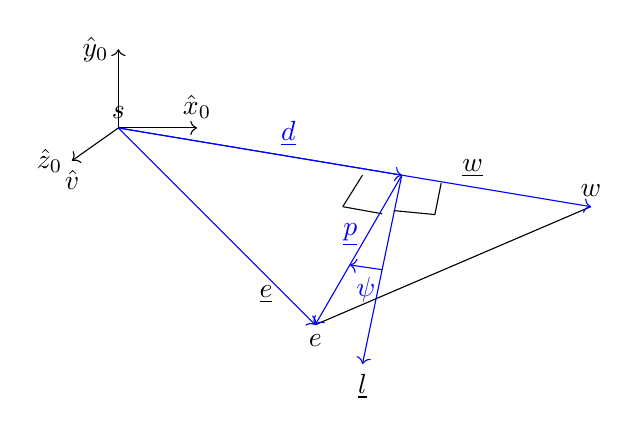
\begin{tikzpicture}
		\coordinate(A) at (2.5, 1.5);
		\coordinate(B) at (1,0);
		\coordinate(C) at (3.5, -2.5);
		\coordinate(D) at (7, -1);
		\coordinate(E) at (8.5, -2.2);
 
        %\draw[-] (A)--(B);
        \draw[->,blue] (B)--(C) node[pos=0.75,below,color=black]{$\underline{e}$};
        \draw[-] (C)--(D);
        %\draw[-] (D)--(E);
        
        \draw[->,blue] (B)--(D) node[pos=0.75,above,color=black]{$\underline{w}$} node[pos=0.6](midway){};
        \draw[->] (B) -- ++(0,1) node[left,color=black]{$\hat{y}_{0}$};
        \draw[->] (B) -- ++(1,0) node[above,color=black]{$\hat{x}_{0}$};
        \draw[->] (B) -- ++(-0.707/1.2,-0.5/1.2) node[left,color=black]{$\hat{z}_{0}$} node[below,color=black]{$\hat{v}$};
        \draw[->,blue] (midway.center)--(C) node[pos=0.4,left]{$\underline{p}$} node[pos=0.6](foo){};
        \draw ($(midway.center)-(0.5, 0)$) -- ($(midway.center)-(0.75, 0.4)$);
        \draw ($(midway.center)-(0.75, 0.4)$) -- ($(midway.center)-(0.25, 0.49)$);
        
        \draw[->,blue] (midway.center)--($(C)+(0.6,-0.5)$) node[pos=0.5](bar){} node[pos=1,below,color=black]{$\underline{l}$};
        \draw ($(midway.center)-(-0.5, 0.1)$) -- ($(midway.center)-(-0.42, 0.5)$);
        \draw ($(midway.center)-(-0.42, 0.5)$) -- ($(midway.center)-(0.1, 0.45)$);
        
        \draw[->,blue] (bar.center) -- (foo.center) node[pos=0.5, below]{$\psi$};
        \draw[->,blue] (B)--(midway.center) node[pos=0.6,above]{$\underline{d}$};

        \draw (B) node[above]{$s$};
        \draw (D) node[above]{$w$};
        \draw (C) node[below]{$e$};

	\end{tikzpicture}
\end{figure}

Define 
\begin{eqnarray}
 \underline{w} & = & \overrightarrow{sw} = \underline{p}_{w}-\underline{p}_{r} \nonumber \\
 \underline{e} & = & \overrightarrow{se} = \underline{p}_{e}-\underline{p}_{s} \nonumber \\
 \hat{x} && \text{is reference vector in base frame} \nonumber \\
 \underline{w}\times\hat{v} && \text{defines the reference plane} \nonumber \\
 \underline{l} && \text{is perpendicular to $\underline{w}$ in reference plane} \nonumber \\
 \underline{d} & = & \hat{w}(\hat{w}^{T}\underline{e}) \nonumber\\
 && \text{$\underline{d}$ is the projection of $\underline{e}$ onto $\underline{w}$}: \nonumber
\end{eqnarray}
\begin{figure}[h!]
	\centering
	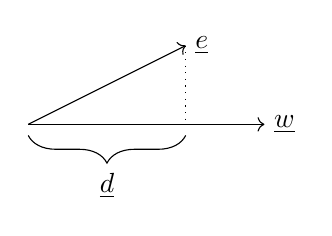
\begin{tikzpicture}
		\coordinate(A) at (0,0);
		\coordinate(B) at (3,0);
		\coordinate(C) at (2,1);
 
        \draw[->] (A)--(B) node[right]{$\underline{w}$};
        \draw[->] (A)--(C) node[right]{$\underline{e}$};
        \draw[dotted] (C)--(2,0);
        \draw [decorate,decoration={brace,amplitude=10pt,mirror,raise=4pt},yshift=0pt] (A) -- (2,0) node[pos=0.5,below=0.5]{$\underline{d}$};
	\end{tikzpicture}
\end{figure}

Then
\begin{eqnarray}
    \underline{p} & = & \underline{e} - \underline{d} = (I-\hat{w}\hat{w}^{T})\underline{e} \nonumber \\
    \underline{l} & = & (\underline{w} \times \hat{\underline{v}}) \times \underline{w} \nonumber
\end{eqnarray}
$\phi$ is the angle between $\underline{l}$ and $\underline{p}$:
\begin{displaymath}
 \tan(\phi) = \frac{\hat{w}^{T}(\underline{l}\times\underline{p})}{\underline{l} \cdot \underline{p}} = \frac{\hat{w}^{T}\left(|\underline{l}||\underline{p}|\sin(\phi)\hat{w}\right)}{|\underline{l}||\underline{p}|\cos(\phi)} = \frac{\sin(\phi)}{\cos(\phi)}\hat{w}^{T}\hat{w} 
\end{displaymath}

$J_{\phi}$ is found by taking the derivative of $\phi$ with respect to $\underline{q}$:
\begin{displaymath}
 \dot{\phi} = J_{\phi}\dot{\underline{q}}
\end{displaymath}
where
\begin{displaymath}
 J_{\phi} = \left[ \begin{array}{ccccccc} x & x & x & x & 0 & 0 & 0 \end{array}\right]
\end{displaymath}
and note that the last three entries do not depend on $n_{5}, n_{6}, n_{7}$. So the extended Jacobian is:
\begin{equation}
 \left[ \begin{array}{c} \dot{\underline{x}} \\ \dot{\phi} \end{array} \right] = \left[ \begin{array}{c} J \\ J_{\phi} \end{array} \right] \dot{\underline{q}}
\end{equation}

\section{Example Problem}

One very common way to use redundant degrees of freedom is to try to keep the manipulator's joints in the middle of their range of motion, so that it's less likely to hit a joint limit. Suppose we wanted to derive a pseudoinverse to make a manipulator with $f>6$ degrees of freedom do this.

We'll define an auxiliary loss term that penalizes angular distance from the center of the robot's range of motion:
\begin{eqnarray}
D & = & \sum_{i=1}^{n} \left( \frac{q_{i}-q_{i}^{\mathrm{mid}}}{q_{i}^{\mathrm{min}}-q_{i}^{\mathrm{max}}}\right)^{2} \\
q^{\mathrm{mid}} & \triangleq & \frac{1}{2}\left( q_{i}^{\mathrm{min}} + q_{i}^{\mathrm{max}} \right)
\end{eqnarray}
where $q_{i}^{\mathrm{min}}$ and $q_{i}^{\mathrm{max}}$ are the minimum and maximum joint angles for joint $i$.
 
 We want to use Resolved Motion Rate Control (RMRC) with a ``custom'' pseudoinverse that uses the extra degrees of freedom to minimize this loss term. What is the RMRC Jacobian relationship for this term --- in other words, what is $\Delta \underline{q}$ with respect to $\Delta\underline{x}$?


\subsection{Answer}
Recall that we derived a general formula to do this in Lecture 12 (specifically, equation 6):
\begin{displaymath}
\Delta\underline{q} = J^{\dag}\Delta\underline{x} + \left[ J^{\dag}J-I\right] \frac{\partial D}{\partial \Delta\underline{q}}^{T}\Delta t
\end{displaymath}
So all we have to do is take the partial of $D$ with respect to each of the joint angles $q_{i}$:
\begin{displaymath}
	\frac{\partial D}{\partial \Delta\underline{q}} = 2\left[
		\begin{matrix}
			\frac{q_{0} - n_{0}^{\mathrm{mid}}}{q_{0}^{\mathrm{min}} - q_{0}^{\mathrm{max}}} & 0 & \dots & 0 \\
			0 & \frac{q_{1} - q_{1}^{\mathrm{mid}}}{q_{1}^{\mathrm{min}} - q_{1}^{\mathrm{max}}} & \dots & 0 \\
			\vdots & \vdots & \ddots & \vdots \\
			0 & 0 & \cdots & \frac{q_{f} - n_{f}^{\mathrm{mid}}}{q_{f}^{\mathrm{min}} - q_{f}^{\mathrm{max}}}
		\end{matrix} \right] \triangleq G
\end{displaymath}
Noting that is diagonal, $D=D^{T}$, and therefore the full RMRC algorithm is:
\begin{displaymath}
\Delta\underline{q} = J^{\dag}\Delta\underline{x} + \left[ J^{\dag}J-I\right]G\ \Delta t
\end{displaymath}

Citation: Hanai, Aaron, Doctoral dissertation, ``A Unified Autonomus Underwater Vehicle--Manipulator System'', University of Hawai`i--Manoa, 2010, pg. 12


\end{document}
